\chapter[Introdução]{Introdução}\label{cap1}
% 	Essa seção aborda sobre o contexto do projeto, o problema a ser resolvido e a metodologia para desenvolvimento do trabalho.
Vibração é conhecida como o movimento oscilatório de um corpo em relação ao um referencial. O número de ciclos vibratórios do movimento por segundo é chamado de frequência, que é medida em Hertz (Hz) \cite[p. 14]{inman}.

A vibração ocorre em todos os corpos, e testes vibratórios são feitos para determinar as frequências naturais de um determinado corpo, afim de evitar ressonância, e, também, para realizar experimentalmente a durabilidade dinâmica de estruturas permitindo obter o comportamento da estrutura perante vibrações \cite[p. 587]{inman}.

	Este trabalho apresenta a proposta de uma bancada para ensaios de vibração mecânica. Assim, neste capítulo são apresentados o problema a ser resolvido, a justificativa e objetivos do projeto.

\section{Descrição do Problema}

    O problema trabalhado neste projeto está representado na Tabela \ref{problem}:

    \begin{table}[h]
        \centering
        \caption{Problema trabalhado no projeto}
        \label{problem}
        \begin{tabular}{|l|l|}
        \hline
        \textbf{O problema de} & Carência de uma bancada de testes de vibração na FGA. \\ \hline
        \textbf{Afeta} & Os alunos de Engenharia Automotiva e Aeroespacial e  da FGA. \\ \hline
        \textbf{Cujo impacto é} & Formação pouco prática. \\ \hline
        \textbf{Uma boa solução seria} & \begin{tabular}[c]{@{}l@{}}um projeto de uma bancada de testes de vibração genérica\\  para testes de diversas estruturas pelos alunos.\end{tabular} \\ \hline
        \end{tabular}
	\end{table}

\section{Justificativa}
    % Melhorar
    A Faculdade UnB Gama conta com excelentes profissionais e alunos, porém possui uma deficiência na infraestrutura e suporte para os alunos. Alguns equipamentos
    necessários para realização de testes faltam no \textit{campus}, o que
    impacta negativamente a formação dos alunos de Engenharia
    Automotiva e Aeroespacial, principalmente.

    Com isso em mente, este projeto foi proposto para suprir a falta de
    um equipamento de testes de vibração na faculdade, área bastante explorada
    em disciplinas dos cursos de Engenharia Automotiva e Aeroespacial.

\section{Objetivos}

% 	Projetar e construir uma mesa vibratória, de frequência ajustável, que possa ser usada em projetos ou pesquisas, feitas pelas engenharias da UnB-FGA, que necessitem de uma superfície que vibra. Bem como desenvolver sistema de sensoriamento, aquisição e visualização das frequência resposta geradas em teste.

    Este trabalho tem por objetivo geral propor o projeto e implementação de uma bancada para ensaios de vibração mecânica para suprir a carência deste equipamento na UnB-FGA, de forma que possa ser utilizado em projetos e pesquisas feitos pelas engenharias do \textit{campus}.

    % 	A bancada vibratória desse projeto será desenvolvida com o intuito de proporcionar o teste de durabilidade dinâmica de estruturas por meio de vibrações que simulam ambientes críticos, os quais a determinada estrutura terá que enfrentar.

   \subsection{Objetivos específicos}
       São objetivos específicos do projeto:
       \begin{itemize}
%         \item Desenvolver interface visual de baixo nível que permita ao usuário organizar e acompanhar a variação da frequência e tempo durante o uso da mesa construída.
%         \item Projetar e construir sistema eletromecânico que proporcione uma faixa de frequência conhecida ao usuário.
%         \item Criar conjunto de sensores que possam medir o efeito da vibração gerada pela mesa, em pontos diferentes, de objetos.
%         \item Criação de protocolo de comunicação para comunicação entre sensores e micro controladores.
%         \item Escrever manual de uso digital da interface de controle.
%         \item Integrar as soluções de cada frente de trabalho.

        \item Projetar e construir o sistema mecânico/estrutural da bancada;
        \item Projetar e construir o sistema eletromecânico de funcionamento da bancada;
        \item Projetar e construir o sistema eletroeletrônico de funcionamento da bancada;
        \item Projetar e construir o sistema de monitoramento e controle do uso da bancada;
        \item Integrar as soluções de cada frente de trabalho.
       \end{itemize}

       No Apêndice \ref{enaoe} encontra-se uma lista que identifica características do produto proposto, esclarecendo um pouco mais o escopo do projeto.

%%%%%%%%%%%%%%%%%%%%% SEÇÃO GERENCIAMENTO
% %%%%%%%%%%%%%%%%%%%%% SEÇÃO GERENCIAMENTO
\chapter{Gerenciamento do Projeto}

Para o gerenciamento do projeto, nas Fases de Concepção e Detalhamento da Solução (01 e 02), foram planejados e documentados, de acordo com os planos estabelecidos pelo PMBOK \cite{pmbok}, as 
áreas de Custos, Aquisições, Recursos Humanos e Riscos. A documentação dos planos podem ser visualizados nos apêndices do 
\href{https://drive.google.com/file/d/0B5InkGKx6O-MR1B3eVYzZFpjQ3c/view?usp=sharing}{Relatório 1}. 

A comunicação da equipe permaneceu como definida nas Fases 01 e 02 e na fase de Projeto e Construção da Solução, foco deste relatório, o plano de gerenciamento de riscos 
(Apêndice \ref{plano_de_riscos}) foi atualizado, assim como o cronograma do projeto e as ferramentas utilizadas. 

\section*{Ferramentas}

\textbf{WhatsApp}:
Aplicativo de mensagens para troca de informações que não necessitam de um encontro presencial.

\textbf{Google Drive\footnote{https://drive.google.com/}}: Serviço de armazenamento de arquivos utilizado para compartilhar todo o material gráfico (documentos, artigos, relatório, \textit{slides}, imagens e etc) utilizados para desenvolvimento do projeto.

\textbf{GitHub\footnote{https://github.com/}}: Ferramenta de gerenciamento de versões utilizada para armazenar e gerenciar 
a escrita do relatório.

\section*{Estrutura Analítica de Projeto}

A EAP apresentada na Figura \ref{eap}, está dividida nas seguintes áreas: Planejamento do Projeto, Interface/Processamento, Eletroeletrônica, Eletromecânica, Estrutura e Encerramento do Projeto. O planejamento e o encerramento contemplam entregáveis relacionados ao projeto propriamente dito, e as demais áreas contemplam os entregáveis relacionados ao produto. As demais áreas foram estabelecidas de acordo com os módulos da bancada. Sendo:

\textbf{Interface/Processamento:} Módulo responsável por tratar da interação com o usuário da bancada, recebendo os parâmetros para controle da bancada e apresentando para o usuário os dados coletados no ensaio.

\textbf{Eletroeletrônica:} Módulo responsável por obter e tratar os sinais brutos dos sensores, disponibilizando dados para os demais módulos. Também é responsável pelo controle da vibração da mesa e interação com os motores.

\textbf{Eletromecânica:} Módulo responsável pelo acionamento do sistema por meio de motores de indução trifásicos, bem como controlar as velocidades e torques exigidos usando-se inversores de frequência afim de gerar a vibração na bancada definida pelo usuário.

\textbf{Estrutura:} Módulo responsável pelos cálculos/simulações estruturais, simulações modais, procura/aquisição dos materiais de construção e fabricação da bancada.

Para cada entregável foi colocado uma \textit{tag} indicando em que ponto de controle (entrega intermediária do projeto) deverá ser entregue, na qual:

\indent \textbf{PC1:} Ponto de Controle 1 - Concepção e Detalhamento da Solução

\indent \textbf{PC2:} Ponto de Controle 2 - Projeto e Construção da Solução

\indent \textbf{PC3:} Ponto de Controle 3 - Integração

\section*{Cronograma}

A partir dos entregáveis estabelecidos na EAP foram definidas as atividades e os prazos. Estes foram acordados entre os líderes de 
cada área e considerando prazo total do projeto (19/08 a 02/12) e as entregas intermediárias (02/09, 04/11 e 30/11).
O cronograma do projeto de forma macro pode ser visto na Figura \ref{cronograma} e o seu detalhamento está disponível
no Google Drive \href{https://drive.google.com/file/d/0B28JW3Vcm0jLdElSSGNPcU4yVEU/view?usp=sharing}{(Cronograma)}.

Para a Fase 03 (Projeto e Construção da Solução) do projeto optou-se por utilizar iterações, como previsto pelo 
\textit{framework} Scrum \cite{scrum}.
As iterações tiveram duração aproximada de 1 semana, 
nas quais as atividades foram planejadas no início da iteração de acordo 
com a macro-atividade estabelecida no cronograma. O planejamento das iterações pode ser visto nas Tabelas \ref{tab:iteracao1},
\ref{tab:iteracao2}, \ref{tab:iteracao3}, \ref{tab:iteracao4} e \ref{tab:iteracao5}.

\begin{figure}[]
\centering
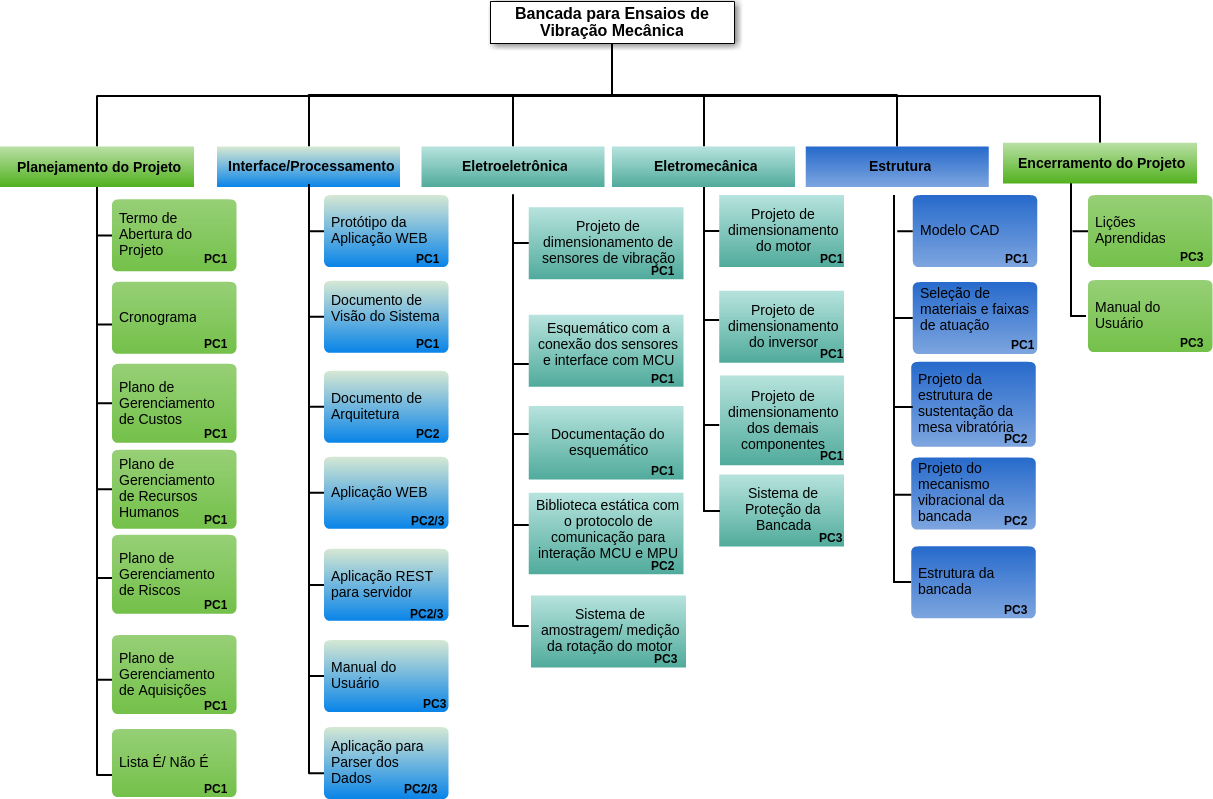
\includegraphics[keepaspectratio=true,scale=0.6,angle=90]{figuras/eap.png}
\caption{EAP do projeto}
\label{eap}
\end{figure}

\begin{figure}[H]
\centering
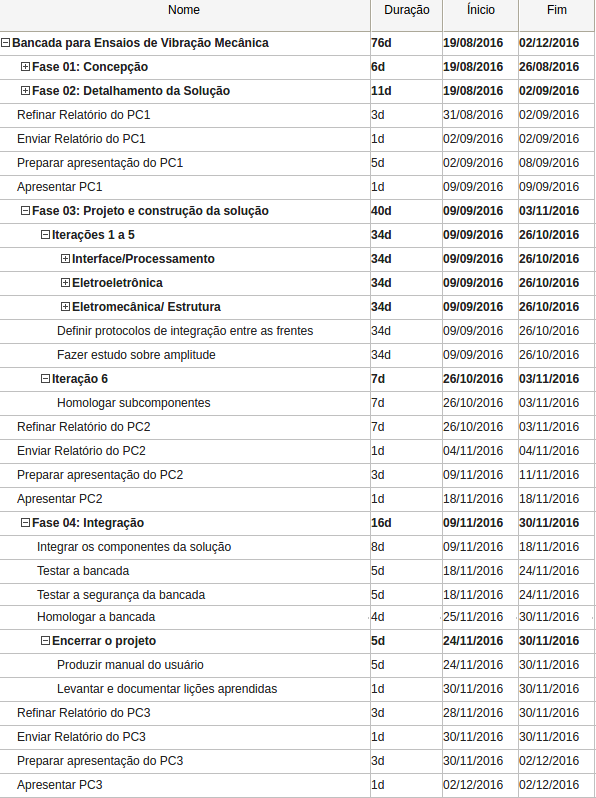
\includegraphics[scale=0.9]{figuras/cronograma_macro.png}
\caption{Cronograma do projeto}
\label{cronograma}
\end{figure}

\begin{table}[H]
\centering
\caption{Atividades - Iteração 1}
\label{tab:iteracao1}
\begin{tabular}{|l|l|}
\hline
\multicolumn{1}{|c|}{\textbf{Início da Iteração}} & \multicolumn{1}{c|}{09/09}                                                                                                                                                                                                                                        \\ \hline
\multicolumn{1}{|c|}{\textbf{Fim da Iteração}}    & \multicolumn{1}{c|}{21/09}                                                                                                                                                                                                                                        \\ \hline
\multicolumn{1}{|c|}{\textbf{Equipe}}             & \multicolumn{1}{c|}{\textbf{Atividades planejadas}}                                                                                                                                                                                                               \\ \hline
\textbf{Estrutura}                                & \begin{tabular}[c]{@{}l@{}}- Cortar Cantoneiras\\ - Soldar Estrutura\end{tabular}                                                                                                                                                                                 \\ \hline
\textbf{Eletromecânica}                           & \begin{tabular}[c]{@{}l@{}}- Realizar ensaio de qualidade com amperímetro, \\ voltímetro e termógrafo\\ - Comprar tomadas e cabos\end{tabular}                                                                                                                    \\ \hline
\textbf{Eletroeletrônica}                         & \begin{tabular}[c]{@{}l@{}}- Estabelecer comunicação entre \\ dois MCUs usando MSP430\\ - Fazer simulação de resposta do microcontrolador\end{tabular}                                                             \\ \hline
\textbf{Interface/Processamento}                  & \begin{tabular}[c]{@{}l@{}}- Modelar banco de dados da aplicação WEB\\ - Modelar banco de dados do REST\\ - Estruturar servidor REST e testar na Raspberry\\ - Implementar Cadastro de Usuário e Login\\ - Implementar Parser dos dados dos sensores\end{tabular} \\ \hline
\end{tabular}
\end{table}

\begin{table}[H]
\centering
\caption{Atividades - Iteração 2}
\label{tab:iteracao2}
\begin{tabular}{|l|l|}
\hline
\multicolumn{1}{|c|}{\textbf{Início da Iteração}} & \multicolumn{1}{c|}{21/09}                                                                                                                            \\ \hline
\multicolumn{1}{|c|}{\textbf{Fim da Iteração}}    & \multicolumn{1}{c|}{28/09}                                                                                                                            \\ \hline
\multicolumn{1}{|c|}{\textbf{Equipe}}             & \multicolumn{1}{c|}{\textbf{Atividades planejadas}}                                                                                                   \\ \hline
\textbf{Estrutura}                                & \begin{tabular}[c]{@{}l@{}}- Definir material da mesa e espessura\\ - Estimar os pesos\\ - Fazer cálculos estruturais\end{tabular}                    \\ \hline
\textbf{Eletromecânica}                           & - Fazer sistema de acionamento do motor                                                                                                               \\ \hline
\textbf{Eletroeletrônica}                         & \begin{tabular}[c]{@{}l@{}}- Trabalhar na estabilidade do módulo UART\\ - Trabalhar na arquitetura do módulo de sensoriamento\end{tabular} \\ \hline
\textbf{Interface/Processamento}                  & \begin{tabular}[c]{@{}l@{}}- Implementar início do experimento\\ - Implementar timer do experimento\\ - Implementar captura dos sensores\end{tabular} \\ \hline
\end{tabular}
\end{table}

\begin{table}[H]
\centering
\caption{Atividades - Iteração 3}
\label{tab:iteracao3}
\begin{tabular}{|l|l|}
\hline
\multicolumn{1}{|c|}{\textbf{Início da Iteração}} & \multicolumn{1}{c|}{28/09}                                                                                                                                                                                                                  \\ \hline
\multicolumn{1}{|c|}{\textbf{Fim da Iteração}}    & \multicolumn{1}{c|}{12/10}                                                                                                                                                                                                                  \\ \hline
\multicolumn{1}{|c|}{\textbf{Equipe}}             & \multicolumn{1}{c|}{\textbf{Atividades planejadas}}                                                                                                                                                                                         \\ \hline
\textbf{Estrutura}                                & \begin{tabular}[c]{@{}l@{}}- Comprar pés\\ - Furar fixação do motor\\ - Fixar apoio dos pés e molas\end{tabular}                                                                                                                            \\ \hline
\textbf{Eletromecânica}                           & - Programar inversor trifásico                                                                                                                                                                                                              \\ \hline
\textbf{Eletroeletrônica}                         & \begin{tabular}[c]{@{}l@{}}- Finalizar módulo UART do BSP \\ - Finalizar conversor PWM-DC\end{tabular} \\ \hline
\textbf{Interface/Processamento}                  & \begin{tabular}[c]{@{}l@{}}- Adaptar parser para prover escalabilidade\\ - Implementar rotina de verificação e passagem\\ dos dados da porta serial \\ - Implementar visualização dos ensaios realizados \end{tabular} \\ \hline
\end{tabular}
\end{table}

\begin{table}[H]
\centering
\caption{Atividades - Iteração 4}
\label{tab:iteracao4}
\begin{tabular}{|l|l|}
\hline
\multicolumn{1}{|c|}{\textbf{Início da Iteração}} & \multicolumn{1}{c|}{14/10}                                                                                                                                                           \\ \hline
\multicolumn{1}{|c|}{\textbf{Fim da Iteração}}    & \multicolumn{1}{c|}{21/10}                                                                                                                                                           \\ \hline
\multicolumn{1}{|c|}{\textbf{Equipe}}             & \multicolumn{1}{c|}{\textbf{Atividades planejadas}}                                                                                                                                  \\ \hline
\textbf{Estrutura}                                & \begin{tabular}[c]{@{}l@{}}- Comprar e instalar molas\\ - Projetar o retentor da correia\\ - Analisar o tampo com os reforços\\ - Fixar o motor\end{tabular}                         \\ \hline
\textbf{Eletromecânica}                           & \begin{tabular}[c]{@{}l@{}}- Fazer teste de integração\\ - Fazer sistema de proteção\\ - Estudar a amplitude \\ - Fixar o motor\end{tabular}                                                            \\ \hline
\textbf{Eletroeletrônica}                         & \begin{tabular}[c]{@{}l@{}}- Testar layouts de controle do inversor\\ - Finalizar BSP\\ - Estudar obtenção da frequência * crítico\\ - Estudar viabilidade da amplitude\end{tabular} \\ \hline
\textbf{Interface/Processamento}                  & \begin{tabular}[c]{@{}l@{}}- Integrar aplicação WEB com o servidor\\ - Implementar população do banco da aplicação\\ - Implementar mais testes \\ - Fazer documento de arquitetura \end{tabular}                          \\ \hline
\end{tabular}
\end{table}

\begin{table}[H]
\centering
\caption{Atividades - Iteração 5}
\label{tab:iteracao5}
\begin{tabular}{|l|l|}
\hline
\multicolumn{1}{|c|}{\textbf{Início da Iteração}} & \multicolumn{1}{c|}{21/10}                                                                                                                                                                                                                                                                                         \\ \hline
\multicolumn{1}{|c|}{\textbf{Fim da Iteração}}    & \multicolumn{1}{c|}{28/10}                                                                                                                                                                                                                                                                                         \\ \hline
\multicolumn{1}{|c|}{\textbf{Equipe}}             & \multicolumn{1}{c|}{\textbf{Atividades planejadas}}                                                                                                                                                                                                                                                                \\ \hline
\textbf{Estrutura}                                & \begin{tabular}[c]{@{}l@{}}- Cortar chapas para produção dos copinhos\\ - Furar chapas\\ - Usinar os copinhos\\ - Cortar copinhos usinados\\ - Soldar copinhos na chapa\\ - Soldar chapa na estrutura\\ - Usinar coroa da polia\end{tabular}                                                                       \\ \hline
\textbf{Eletromecânica}                           & \begin{tabular}[c]{@{}l@{}}- Montar cabeamento do inversor\\ - Montar cabeamento do motor\end{tabular}                                                                                                                                                                                                             \\ \hline
\textbf{Eletroeletrônica}                         & \begin{tabular}[c]{@{}l@{}}- Finalizar circuito de contagem de unidades \\ de expansão\\ - Fechar módulo I2C do BSP\end{tabular}                                                                                                                                                                                   \\ \hline
\textbf{Interface/Processamento}                  & \begin{tabular}[c]{@{}l@{}}- Concluir fluxo de ida e de volta da aplicação\\       - Ler sensores e dados dos sensores\\ - Implementar pausa do ensaio a cada mudança de \\ frequência\\ - Adaptar modelagem do banco do REST\\ - Definir técnica de processamento dos dados\\ - Otimizar a aplicação\end{tabular} \\ \hline
\end{tabular}
\end{table}


\section{Acompanhamento das Aquisições}

Na Tabela \ref{tab:acompanhamento_custos} podem ser vistas as aquisições realizadas durante a Fase 03 do projeto.

\begin{table}[H]
\centering
\caption{Aquisições do projeto}
\label{tab:acompanhamento_custos}
\begin{tabular}{|l|c|l|}
\hline
\multicolumn{1}{|c|}{\textbf{Item adquirido}} & \textbf{Quantidade} & \multicolumn{1}{c|}{\textbf{Custo Unitário}} \\ \hline
Inversor trifásico                            & 1                   & R\$ 400,00                                   \\ \hline
4m de cabo de 5 polos                         & 1                   & R\$ 15                                       \\ \hline
1 tomada stack 3f+n+t 32a                     & 1                   & R\$ 35                                       \\ \hline
1 tomada stack 3f+n+t 16a macho (plug)        & 1                   & R\$ 20                                       \\ \hline
1 tomada stack 3f+n+t 16a fêmea               & 1                   & R\$ 20                                       \\ \hline
4m de cabo de 4 polos 3f+t                    & 1                   & R\$ 15                                       \\ \hline
Terminais pré-isolados                        & 10                  & R\$ 5                                        \\ \hline
Acelerômetro adxl335 triaxial                 & 6                   & R\$ 19.55                                    \\ \hline
                                              &                     &                                              \\ \hline
\multicolumn{2}{|c|}{\textbf{Orçamento}}                            &                                              \\ \hline
\multicolumn{2}{|c|}{\textbf{Custo total}}                          &                                              \\ \hline
\end{tabular}
\end{table}

%%%%%%%%%%%%%%%%%%%%% FIM SEÇÃO GERENCIAMENTO

\chapter{Gerenciamento do Projeto}

Para o gerenciamento do projeto foram planejados os Custos (Apêndice \ref{plano_de_custos}), Aquisições (Apêndice \ref{plano_de_aquisicoes}), Recursos Humanos (Apêndice \ref{plano_de_rh}) e Riscos (Apêndice \ref{plano_de_riscos}), estes foram documentados de acordo com os planos estabelecidos pelo PMBOK \cite{pmbok}.
Além disso foram estabelecidas as formas de comunicação, as ferramentas para gestão e documentação do projeto que serão utilizadas, os entregáveis, as atividades, responsáveis e prazos.

\section*{Comunicação da equipe}
A equipe possui reuniões presenciais duas vezes pela semana, estabelecidas da seguinte forma:
\begin{center}
  \begin{itemize}
      \item Quartas (16h às 18h)
      \item Sextas (14h às 18h)
  \end{itemize}
\end{center}

Essas reuniões são utilizadas para discussões acerca do andamento do projeto e para tomada de decisões. Nos horários estabelecidos também ocorre a execução das demais atividades do projeto.
Para a comunicação a distância é utilizado o aplicativo de mensagens WhatsApp\footnote{https://www.whatsapp.com/}.

\section*{Ferramentas}

\textbf{WhatsApp}:
Aplicativo de mensagens para troca de informações que não necessitam de um encontro presencial.

\textbf{Google Drive\footnote{https://drive.google.com/}}: Serviço de armazenamento de arquivos utilizado para compartilhar todo o material gráfico (documentos, artigos, relatório, \textit{slides}, imagens e etc) utilizados para desenvolvimento do projeto.

\textbf{Trello\footnote{https://trello.com/}}:
Ferramenta para organização de tarefas do projeto de cada módulo. Também utilizada para gerenciamento dos requisitos do módulo de Interface/Processamento (\textit{Backlog} do Produto).

\textbf{Overleaf\footnote{https://www.overleaf.com/}}:
Ferramenta online de edição colaborativa de Latex\footnote{https://www.latex-project.org/} utilizada para escrita do relatório do projeto.

\section*{Estrutura Analítica de Projeto}

A EAP apresentada na Figura \ref{eap}, está dividida nas seguintes áreas: Planejamento do Projeto, Interface/Processamento, Eletroeletrônica, Eletromecânica, Estrutura e Encerramento do Projeto. O planejamento e o encerramento contemplam entregáveis relacionados ao projeto propriamente dito, e as demais áreas contemplam os entregáveis relacionados ao produto. As demais áreas foram estabelecidas de acordo com os módulos da bancada. Sendo:

\textbf{Interface/Processamento:} Módulo responsável por tratar da interação com o usuário da bancada, recebendo os parâmetros para controle da bancada e apresentando para o usuário os dados coletados no ensaio.

\textbf{Eletroeletrônica:} Módulo responsável por obter e tratar os sinais brutos dos sensores, disponibilizando dados para os demais módulos. Também é responsável pelo controle da vibração da mesa e interação com os motores.

\textbf{Eletromecânica:} Módulo responsável pelo acionamento do sistema por meio de motores de indução trifásicos, bem como controlar as velocidades e torques exigidos usando-se inversores de frequência afim de gerar a vibração na bancada definida pelo usuário.

\textbf{Estrutura:} Módulo responsável pelos cálculos/simulações estruturais, simulações modais, procura/aquisição dos materiais de construção e fabricação da bancada.

Para cada entregável foi colocado uma \textit{tag} indicando em que ponto de controle (entrega intermediária do projeto) deverá ser entregue, na qual:

\indent \textbf{PC1:} Ponto de Controle 1 - Concepção de Detalhamento da Solução

\indent \textbf{PC2:} Ponto de Controle 2 - Projeto e Construção da Solução

\indent \textbf{PC3:} Ponto de Controle 3 - Integração

\section*{Cronograma}

A partir dos entregáveis estabelecidos na EAP foram definidas as atividades e os prazos. Estes foram acordados entre os líderes de cada área e considerando prazo total do projeto (19/08 a 02/12) e as entregas intermediárias (02/09, 04/11 e 30/11).

Para a Fase 03 do projeto optou-se por utilizar iterações, como prevista pelo \textit{framework} Scrum\footnote{http://www.scrumguides.org/docs/scrumguide/v1/Scrum-Guide-Portuguese-BR.pdf}. As iterações serão de 1 semana, nas quais as atividades e responsáveis serão planejadas no início da iteração de acordo com a macro-atividade estabelecida no cronograma.
O cronograma do projeto de forma macro pode ser visto na Figura \ref{cronograma}. O cronograma detalhado está disponível no Apêndice \ref{cronograma_detalhado}.

\begin{figure}[!ht]
\centering
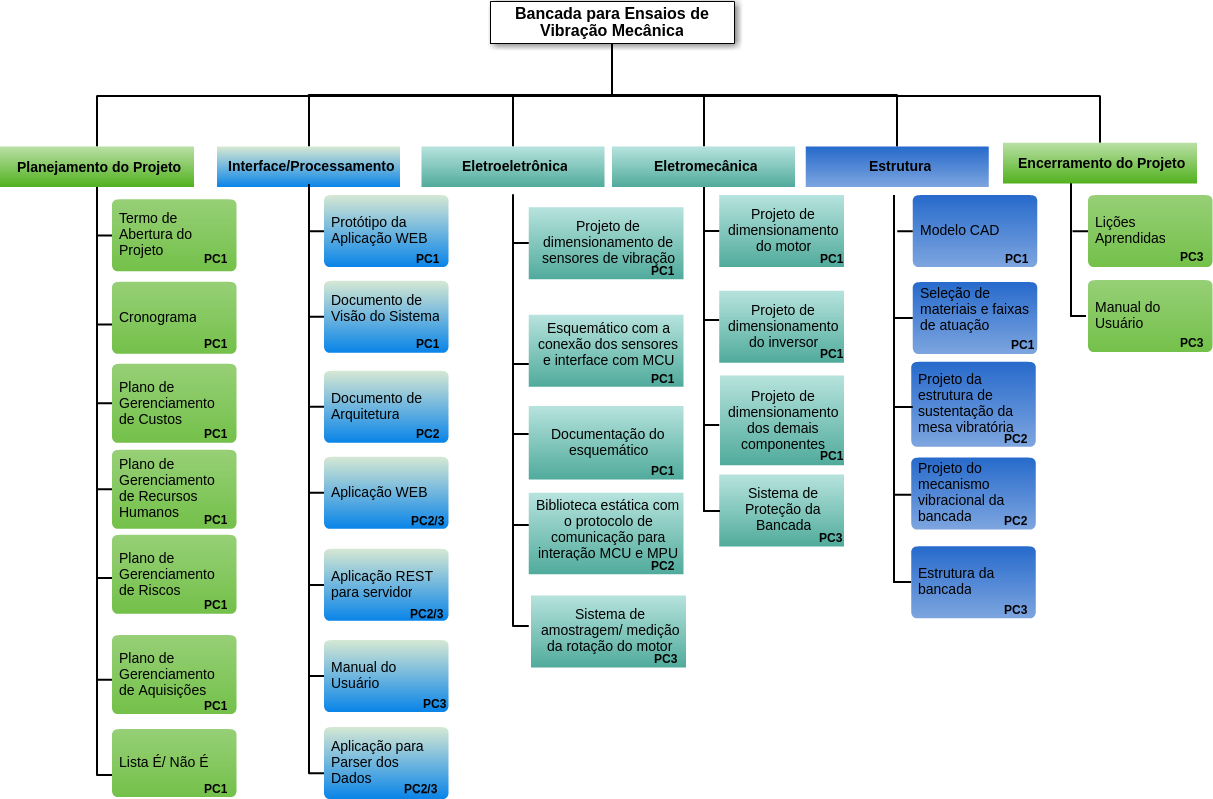
\includegraphics[keepaspectratio=true,scale=0.6,angle=90]{figuras/eap.png}
\caption{EAP do projeto}
\label{eap}
\end{figure}

\begin{figure}[!ht]
\centering
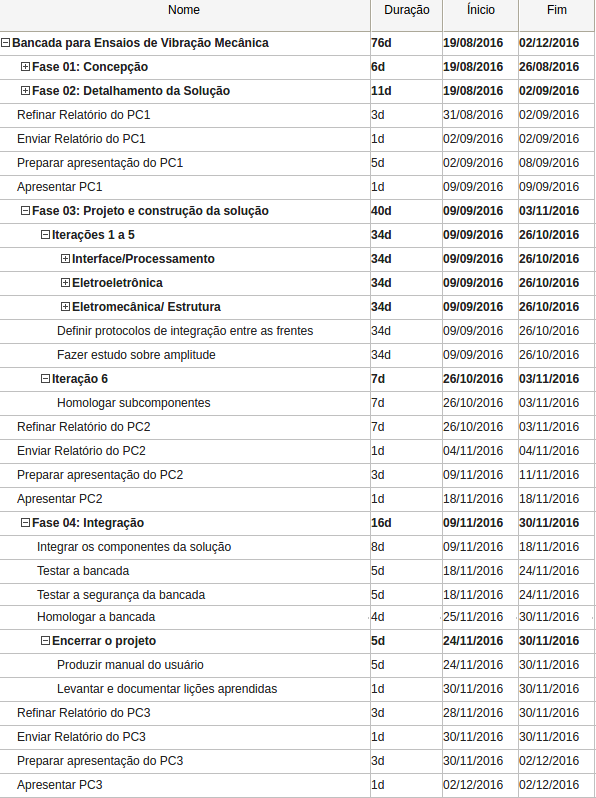
\includegraphics[scale=0.9]{figuras/cronograma_macro.png}
\caption{Cronograma do projeto}
\label{cronograma}
\end{figure}

%%%%%%%%%%%%%%%%%%%%% FIM SEÇÃO GERENCIAMENTO
